\documentclass[12pt,a4paper]{article}
\usepackage[utf8]{inputenc}
\usepackage[german]{babel}
\usepackage[T1]{fontenc}
\usepackage{amsmath}
\usepackage{amsfonts}
\usepackage{amssymb}
\usepackage{wrapfig}
\usepackage{graphicx}
\usepackage{hyperref}
\usepackage[left=2cm,right=2cm,top=2cm,bottom=2cm]{geometry}
\usepackage[dvipsnames]{xcolor}
\author{Gerhard Hofmann}
\title{Simulation eines Nahwärmesystems mit solarthermischer Energiequelle und Erdsonden-Wärmespeicher}
\begin{document}
\maketitle
\tableofcontents
\section{Kurzfassung}
Nahwärmesysteme mit solarthermischer Energiequelle und Erdsonden-Wärmespeicher sind ein vielversprechendes Konzept für die Wärmewende, d.h. für die Wärmeversorgung von Büro- und Wohnhäusern ohne fossile Brennstoffe und mit minimalem Stromeinsatz.\\
Ein solches System besteht aus mehreren Komponenten, die gut aufeinander abgestimmt sein müssen. Als Komponenten betrachten wir:\begin{itemize}
\item Solarthermiefeld
\item Erdsonden-Wärmespeicher
\item Pufferspeicher
\item Wärmeverbraucher
\item Hausübergabestation
\item Nahwärmeleitungen
\item Wärmepumpen
\end{itemize}
Manche dieser Komponenten sind in einem bestimmten Szenario bereits vorgegeben, andere müssen noch dimensioniert werden. 
Es wird angestrebt, eine möglichst hohe solare Deckungsrate bei der Wärmeversorgung zu erreichen. Dazu kann man mit der hier vorgestellten Software \texttt{DistrictHeating} die verschiedenen noch freien Parameter (z.B. Abstand der Erdsonden zueinander, Vorlauftemperatur im Netz u.v.m.) variieren und nach einer Simulation über den Jahresverlauf z.B. den Stromverbrauch der Wärmepumpen feststellen.\\
Angeregt wurde die Entwicklung der Simulation \texttt{DistrictHeating} durch die Dissertation \emph{\glqq Object-oriented modelling of solar district heating grids with underground thermal energy storage\grqq} \footnote{\url{https://tubiblio.ulb.tu-darmstadt.de/133074/}} von Julian Formhals, in der die Simulation eines ebensolchen Nahwärmesystems basierend auf Modelica beschrieben wird. Diese Simulation von Julian Formhals ist weitaus realistischer als \texttt{DistrictHeating}, benötigt jedoch auch wesentlich mehr Rechenzeit. Somit ist es kaum möglich mehrere Parameter über Testreihen zu verändern um eine optimale Konfiguration zu finden.
\section{Einleitung}
Das \texttt{DistrictHeating} zugrunde liegende physikalische Konzept besteht aus einem Nahwärme-Leitungsnetz mit zwei oder drei Leitungen, die in der Straße verlegt werden und an die die verschiedenen Komponenten angeschlossen sind. Die einzelnen Komponenten können dem Netz Wärme entziehen oder Wärme zuführen.
\section{Die Simulation}
\texttt{DistrictHeating} ist in \texttt{C\#} geschrieben und läuft unter .NET. Die Applikation enthält eine Benutzeroberfläche, mit deren Hilfe die Komponenten zusammengestellt und definiert werden können. Die Möglichkeiten sind weit entfernt von dem, was in Modelica möglich ist. Es ist vielmehr genau zugeschnitten auf eine Anlage mit einem Solarthermiefeld, einem Erdsonden-Wärmespeicher, einem Pufferspeicher, verschiedenen Wärmeverbrauchern, Nahwärmeleitungen und Wärmepumpen.
\subsection{Komponenten} Die einzelnen Komponenten sind als Klassen implementiert. Im wesentlichen ist es die Aufgabe der Komponenten zu einem gegebenen Zeitpunkt zu berechnen, mit welcher Leistung dem System gerade Energie zugeführt oder entnommen wird und wie viel zusätzlicher Strom (z.B. für eine Wärmepumpe) verwendet wird. Dazu muss die Komponente folgende Werte bestimmen:
\begin{description}
\item[Volumenstrom (\texttt{out double volumetricFlowRate}) in $\frac{m^3}{s}$]
\item[Temperaturdifferenz (\texttt{out double deltaT}) in $K$]
\item[Eingangsleitung (\texttt{out Pipe fromPipe})]
\item[Ausgangsleitung (\texttt{out Pipe toPipe})]
\item[Elektrische Leistung (\texttt{out double electricPower}) in $W$]
\end{description}
\texttt{Pipe} ist einer der folgenden Werte: \texttt{enum Pipe \{ returnPipe, warmPipe, hotPipe \}}.
Es sind Anlagen simulierbar mit zwei Leitungen (warmer Vorlauf und kalter Rücklauf für Verbraucher, für Erzeuger ist die Richtung umgekehrt) oder drei Leitungen (im Winter zwei verschiedene Temperaturen für Vorlauf, der wärmere für Warmwasser und Heizkörperheizung mit garantierten 50°C, im Sommer 50°C für Warmwasser und 5°C zum Kühlen, und jeweils ein Rücklauf). Im Dreileitungssystem entscheidet die Komponente, aus welcher Leitung sie das Wasser zieht und in welche Leitung sie das thermisch veränderte Wasser wieder abgibt.
Die Leistung wird definiert durch einen Volumenstrom $\frac{m^3}{s}$ des Wärmeträgers (Wassers) in den Leitungen und einer Temperaturdifferenz $\Delta T$ zwischen dem entnommenen und dem wieder zugeführten Wasser.
\subsection{Die Anlage (\texttt{class Plant})}
Die Anlage (\texttt{class Plant}) ist das zentrale und singuläre Objekt der Simulation. Sie ist selbst keine Komponente. Sie kennt den Zustand der Leitungen, d.h. die Temperatur des Wassers in den Leitungen. Darüber hinaus kennt sie den Zeitpunkt, an dem sich die Simulation gerade befindet und hält eine Liste aller Komponenten.\\
Die Simulation fragt alle Komponenten der Reihe nach ab, mit welcher Leistung sie gerade arbeiten und verändert entsprechend die Temperatur im Leitungsnetz. Die Geometrie des Leitungsnetzes, also an welcher Stelle die einzelnen Komponenten angeschlossen sind, oder die Auslegung als Ring oder Netz, wird nicht berücksichtigt. Lediglich die Länge, das Wasservolumen und die Dämmwerte sind gegeben und werden entsprechend berücksichtigt.
\subsection{Die Heizung (\texttt{class HeatingConsumer})}
Die Heizung (\texttt{class HeatingConsumer}) ist der typische Wärmeverbraucher. In ihrer Definition sind folgende Eigenschaften gesetzt:
\begin{description}
\item[Vorlauftemperatur (\texttt{double[] SupplyTemp}):] acht Werte, die die Vorlauftemperatur zwischen -20°C und +20°C in 5° Schritten definieren. Zwischenwerte werden linear interpoliert.
\item[Gesamtverbrauch pro Jahr (\texttt{double PowerConsumptionPerYear}) in $J$.]
\item[Die Temperaturen (\texttt{double DayTemperature, double NightTemperature}):] die gewünschte Raumtemperatur.
\item[Nachtabsenkung (\texttt{int DayStartHour, int DayEndHour}):]
 Start- und Endzeit für die Tagestemperatur. Dazwischen ist Nachtabsenkung.
\item[Gütegrad der Wärmepumpe (\texttt{double HeatPumpEfficiency}):]
Die Effizienz der Wärmepumpe, die zum Einsatz kommt, wenn die Temperatur aus dem Nahwärmenetz kleiner ist als die gewünschte Vorlauftemperatur.
\end{description}
Die Heizung greift auf die Wetterdaten zu. Die benötigte Leistung wird proportional zur Differenz aus Vorlauftemperatur und der Außentemperatur gesetzt. Der Faktor für die Proportionalität wird  so bestimmt, dass der Jahresverbrauch den vorgegebenen Wert erreicht. Zum Test habe ich aus den Wetterdaten des DWD \footnote{Deutscher Wetterdienst, Klimadaten zum direkten Download (Gießen/Wettenberg) \url{https://opendata.dwd.de/climate_environment/CDC/observations_germany/}} die monatlichen Verbräuche bestimmt und mit den zu erwartenden gemäß \emph{statista}\footnote{siehe Struktur des jährlichen Erdgasverbrauchs in deutschen Haushalten nach Monaten \url{https://de.statista.com/statistik/daten/studie/160067/umfrage/verbrauch-von-heizenergie-nach-monaten/}} verglichen. Siehe Tabelle \ref{Monatsverbrauch}
\begin{table}[h]\scriptsize \centering
\begin{tabular}[h]{c|c|c|c|c|c|c|c|c|c|c|c|c}
Jahr & Jan & Feb & Mär & Apr & Mai & Jun & Jul & Aug & Sep & Okt & Nov & Dez \\
\hline
Avg & 16.1 & 13 & 12.5 & 8.1 & 3.5 & 2.2 & 1.7 & 1.6 & 5.2 & 8.4 & 12.2 & 15.5 \\
\hline
2000 & 16\% & 13.1\% & 12.2\% & 8.2\% & 3.8\% & 2.8\% & 3.1\% & 0.8\% & 4.7\% & 8.2\% & 12.2\% & 14.8\% \\
2001 & 15.6\% & 12.7\% & 12\% & 9.6\% & 3.3\% & 4\% & 1\% & 0.9\% & 6.3\% & 6\% & 13.1\% & 15.6\% \\
2002 & 15.5\% & 12\% & 12.2\% & 9.3\% & 5.1\% & 1.5\% & 1.5\% & 0.7\% & 5.6\% & 9.5\% & 12\% & 15.1\% \\
2003 & 16.3\% & 15.6\% & 10.9\% & 8.5\% & 4.3\% & 0.9\% & 0.6\% & 0.7\% & 4.9\% & 10.7\% & 10.8\% & 15.6\% \\
2004 & 14.9\% & 12.8\% & 12.5\% & 7.9\% & 5.9\% & 3.1\% & 1.8\% & 1.2\% & 3.8\% & 7.7\% & 12.5\% & 15.9\% \\
2005 & 14.6\% & 15.7\% & 11.8\% & 7.6\% & 5.5\% & 2.6\% & 1.4\% & 2\% & 4\% & 7\% & 12.4\% & 15.3\% \\
2006 & 17.9\% & 14.4\% & 14.7\% & 9.6\% & 5.1\% & 2.8\% & 0.2\% & 3.6\% & 2.5\% & 6.1\% & 10\% & 13.2\% \\
2007 & 12.6\% & 13\% & 11.9\% & 6.3\% & 4.2\% & 2.1\% & 2.5\% & 2.3\% & 6.1\% & 9.7\% & 13.4\% & 16\% \\
2008 & 13.1\% & 12.8\% & 12.8\% & 9.8\% & 3.5\% & 2.3\% & 1.5\% & 1.4\% & 6.2\% & 9.1\% & 12.1\% & 15.4\% \\
2009 & 18.1\% & 13.7\% & 12.2\% & 6.5\% & 4.5\% & 4.4\% & 1.1\% & 1.2\% & 3.9\% & 9\% & 9.9\% & 15.4\% \\
2010 & 16\% & 12.9\% & 11.1\% & 7.3\% & 6.7\% & 2.3\% & 0.7\% & 2.1\% & 5.3\% & 8.6\% & 10.6\% & 16.5\% \\
2011 & 15.2\% & 14.1\% & 11.8\% & 6.3\% & 4.5\% & 3\% & 2.6\% & 1.7\% & 4.6\% & 9.3\% & 13.3\% & 13.6\% \\
2012 & 14.8\% & 15.4\% & 10.1\% & 8.8\% & 4.1\% & 3.3\% & 2\% & 1.1\% & 5.6\% & 9.3\% & 11.9\% & 13.6\% \\
2013 & 15.3\% & 14.4\% & 14.7\% & 8.3\% & 6.3\% & 3.4\% & 0.5\% & 1.2\% & 4.6\% & 6.8\% & 12\% & 12.4\% \\
2014 & 14.9\% & 13\% & 11.6\% & 7.3\% & 6.2\% & 3.8\% & 0.8\% & 3.4\% & 3.6\% & 7.2\% & 12.5\% & 15.6\% \\
2015 & 15\% & 14.5\% & 12.8\% & 8.8\% & 6\% & 2.7\% & 1.1\% & 1.1\% & 5.4\% & 9.7\% & 11\% & 11.9\% \\
2016 & 14.5\% & 12.9\% & 13.3\% & 9.8\% & 4.4\% & 2.5\% & 1.1\% & 1.2\% & 2.7\% & 9\% & 13.1\% & 15.5\% \\
2017 & 17.9\% & 13\% & 10\% & 10\% & 5\% & 1.7\% & 1.5\% & 1.5\% & 5.3\% & 8\% & 12.4\% & 13.6\% \\
2018 & 14.2\% & 17.6\% & 15.1\% & 6.5\% & 2.9\% & 2\% & 0.5\% & 1\% & 4.8\% & 8.5\% & 12.4\% & 14.4\% \\
2019 & 15.8\% & 13.1\% & 11.1\% & 8.3\% & 7.4\% & 1.2\% & 1.3\% & 1.1\% & 5\% & 8.4\% & 12.9\% & 14.4\% \\
2020 & 14.9\% & 13.1\% & 12.4\% & 8.1\% & 6.6\% & 2.6\% & 1.1\% & 0.8\% & 4.9\% & 8.6\% & 12.7\% & 14.4\% \\
2021 & 14.2\% & 13.8\% & 12.2\% & 11.1\% & 7.2\% & 1.2\% & 0.9\% & 2.2\% & 3.6\% & 8.8\% & 11.8\% & 12.9\% \\
\end{tabular}
\caption{Relativer Monatsverbrauch für verschiedene Jahre der Wetterdaten}
\label{Monatsverbrauch}
\end{table}
Da diese Daten gut passen, kann es also bei o.g. linearen Faktor bleiben. Die Heizung ist also nach dem erwarteten Ergebnis modelliert, nicht nach ihren physikalischen Gegebenheiten.\\
Wenn die Temperatur aus dem Nahwärmenetz kleiner ist als die geforderte Vorlauftemperatur, springt die Wärmepumpe ein.
Sei $T_{n}$ die Netztemperatur, $T_{v}$ die benötigte Vorlauftemperatur, $\eta_{hp}$ der Gütegrad der Wärmepumpe und $P_{th}$ die benötigte thermische Leistung (berechnet aus Wetterdaten und Jahresverbrauch), so berechnet sich die benötigte Entzugsleistung aus dem Netz $P_{n}$ und die elektrische Leistung $P_{el}$ wie folgt:
\begin{align}
    COP &= \eta_{hp}\cdot \frac{T_{v}}{T_{v}-T_{n}}\\
    P_{n} &= \frac{COP-1}{COP}\cdot P_{th}\\
    P_{el} &= \frac{1}{COP}\cdot P_{th}
\end{align}
Wenn die Netztemperatur groß genug ist, ist $P_{n}=P_{th}$.
Die Leistung $P_{n}$ muss in einen Volumenstrom $Q$ und Temperaturdifferenz $\Delta T$ umgerechnet werden:
\begin{align}
    Q &= \frac{P_{th}}{4.2\cdot\Delta T}
\end{align}
\colorbox{Yellow}{$\Delta T$  wird z.Z. fest auf $10$ gesetzt, vielleicht gibt es eine realistischere Abschätzung oder Formel.}
\subsection{Das Sonnenkollektor Feld (\texttt{class SolarThermalCollector})}
Das Feld der Sonnenkollektoren ist die Wärmequelle für das System. Es ist definiert durch folgende Eigenschaften:
\begin{description}
\item[Fläche (\texttt{double Area}):] Die Grundfläche des Feldes. 
\item[Wirkungsgrad (\texttt{double Efficiency}):] 
\item[Minimaler Volumenstrom (\texttt{double minVolumetricFlowRate}):]
\item[Maximaler Volumenstrom (\texttt{double maxVolumetricFlowRate}):]
\item[Ausgangstemperatur (\texttt{double prefferedOutTemperature}):] 
\end{description}
Die Größe des Feldes wird als Grundfläche gemessen. Die schräge Aufstellung der Kollektoren, mit der auch eine Verkleinerung der Kollektorenfläche einhergeht, wird nicht berücksichtigt. Ebenso die gegenseitige Verschattung der Module oder Verringerung der Fläche durch hohen Sonnenstand bleibt unberücksichtigt. \\
Der Wirkungsgrad wird fest vorgegeben. Denkbar wäre es, ihn mittels einer Formel aus Eingangstemperatur, Umgebungstemperatur und Volumenstrom zu bestimmen.\\
Die Steuerung kann automatisch von statten gehen und ist durch die Werte für die Eigenschaften minimaler bzw. maximaler Volumenstrom und gewünschter Ausgangstemperatur festgelegt: Sobald genügend Strahlung auf die Kollektoren triff, so dass bei dem minimalen Volumenstrom die Temperatur am Ausgang der Kollektoren die Temperatur der Einspeiseleitung überschreitet arbeitet die Pumpe. Es wird dann versucht die gewünschte Ausgangstemperatur zu erreichen, ohne den minimalen Volumenstrom zu unterschreiten. Nimmt die Sonneneinstrahlung zu, so steigert die Pumpe ihre Leistung bis zum maximalen Volumenstrom, um die gewünschte Ausgangstemperatur zu erreichen. Überschreitet die Strahlung einen gewissen Wert, so geht die Ausgangstemperatur über den gewünschten Wert hinaus, wobei der maximale Volumenstrom eingehalten wird.\\
Der Volumenstrom kann auch von der zentralen Steuerung eingestellt (überschrieben) werden, die die Belange der gesamten Anlage berücksichtigt.

\subsection{Der Erdsonden-Wärmespeicher (\texttt{class ThermalStorage})}
Der Erdsonden-Wärmespeicher ist das zentrale und zugleich komplexeste Element der Simulation. Ziel ist es, das Verhalten des Erdsondenspeichers möglichst realitätsnah zu simulieren. D.h. bei gegebenem Volumenstrom und Temperatur die Temperaturzunahme bzw. Abnahme zu berechnen, wobei natürlich der Ladezustand des Speichers wesentlichen Einfluss nimmt. Der Ladezustand ist natürlich kein einfacher Wert, sondern durch räumliche Temperaturverteilung im Speicher gegeben.
\subsubsection{Grundlage der Simulation}
Im Wesentlichen wird die Temperaturverteilung als zweidimensionales Problem behandelt gemäß der Wärmeleitungsgleichung:
 \begin{align}
 \frac{\partial T}{\partial t} = \alpha \left( \frac{\partial^2 T}{\partial x^2} + \frac{\partial^2 T}{\partial y^2} \right)
 \end{align}
Dabei steht $T$ für die Temperatur, $t$ für die Zeit, $\alpha$ für die thermische Diffusivitätskonstante ($\alpha=\frac{\lambda}{\rho c}$, wobei $\lambda$ die Wärmeleitfähigkeit, $c$ die spezifischen Wärmekapazität und $\rho$ die Dichte darstellt) und $x$ und $y$ für die räumlichen Koordinaten in der Ebene.
Mit Hilfe des impliziten \href{https://de.wikipedia.org/wiki/Crank-Nicolson-Verfahren#Beispiel:_Zweidimensionale_Diffusion}{Crank-Nicolson-Verfahrens} kann dann die Temperaturverteilung in der aufgerasterten Ebene in Zeitschritten berechnet werden.
 \begin{align}
 \begin{split}
\frac{T_{i,j}^{n+1} - T_{i,j}^n}{\Delta t} = \frac{\alpha}{2} \left[ \frac{T_{i+1,j}^{n+1} - 2T_{i,j}^{n+1} + T_{i-1,j}^{n+1}}{\Delta x^2} + \frac{T_{i,j+1}^{n+1} - 2T_{i,j}^{n+1} + T_{i,j-1}^{n+1}}{\Delta y^2} \right. \\
\left. + \frac{T_{i+1,j}^n - 2T_{i,j}^n + T_{i-1,j}^n}{\Delta x^2} + \frac{T_{i,j+1}^n - 2T_{i,j}^n + T_{i,j-1}^n}{\Delta y^2} \right]
\end{split}
\end{align}
$T_{i,j}^{n+1}$ ist die Temperatur an der Stelle $(i,j)$ zum Zeitpunkt $n+1$. Das ist recht aufwendig, da für jede Stelle eine lineare Gleichung mit 5 Unbekannten zu lösen ist, insgesamt also ein großes lineares Gleichungssystem.\\
Einfacher wird es mit dem expliziten Verfahren: hierbei berücksichtigt man für jede Stelle nur die aktuellen Temperaturen der Nachbarzellen und nicht die Temperaturen des nächsten Zeitschritts. Die Gleichung lautet dann 
\begin{align}
T_{i,j}^{n+1}  = \alpha \Delta t \left[ 
\frac{T_{i+1,j}^n - 2T_{i,j}^n + T_{i-1,j}^n}{\Delta x^2} + \frac{T_{i,j+1}^n - 2T_{i,j}^n + T_{i,j-1}^n}{\Delta y^2} \right] + T_{i,j}^n
\end{align}
Somit sind alle Temperaturen für den nächsten Zeitschritt direkt und unabhängig voneinander aus den Temperaturen des aktuellen Zeitschritts zu berechnen.\\
Diese explizite Methode liefert bei den Gegebenheiten, wie wir sie in einem Erdsondenfeld wiederfinden, sehr genau das gleiche Ergebnis wie die implizite Methode aber um Größenordnungen schneller. \\
\begin{sloppypar}
In einem Testbeispiel waren die Zeitschritte $\Delta t = 3600s$ und die Diffusivitätskonstante \mbox{$\alpha = \frac{\lambda}{c\rho} = \frac{2.3\frac{W}{m \cdot K}}{700\frac{J}{kg \cdot K} \cdot 2200\frac{kg}{m^3}} \approx 1.5\cdot 10^{-6}\frac{s}{m^2}$} (das sind Werte für Sandstein). Das räumliche Raster betrug \mbox{$\Delta x = \Delta y = 1m$}. Das ganze Feld wurde mit $100 \cdot 100$ Feldern simuliert, wobei fast alle Felder auf $10$~°C eingestellt wurden und einzelne Felder mit $50$~°C angenommen wurden. Es wurden 1000 Schritte berechnet. Die Unterschiede zwischen der expliziten und der impliziten Methode betrugen weniger als $10^{-3}K$.
\end{sloppypar}
Des Weiteren wurde überprüft, dass die Gesamtenergie des Feldes während der Simulation unverändert bleibt. Auch Verkürzung der Zeitschritte auf $360s$ oder feinere Rasteraufteilung auf $25cm$ brachten die gleichen Ergebnisse.
\subsubsection{Hexagonale Aufteilung des Erdsondenfeldes}
\begin{wrapfigure}{r}{0.35\textwidth}
  \centering
  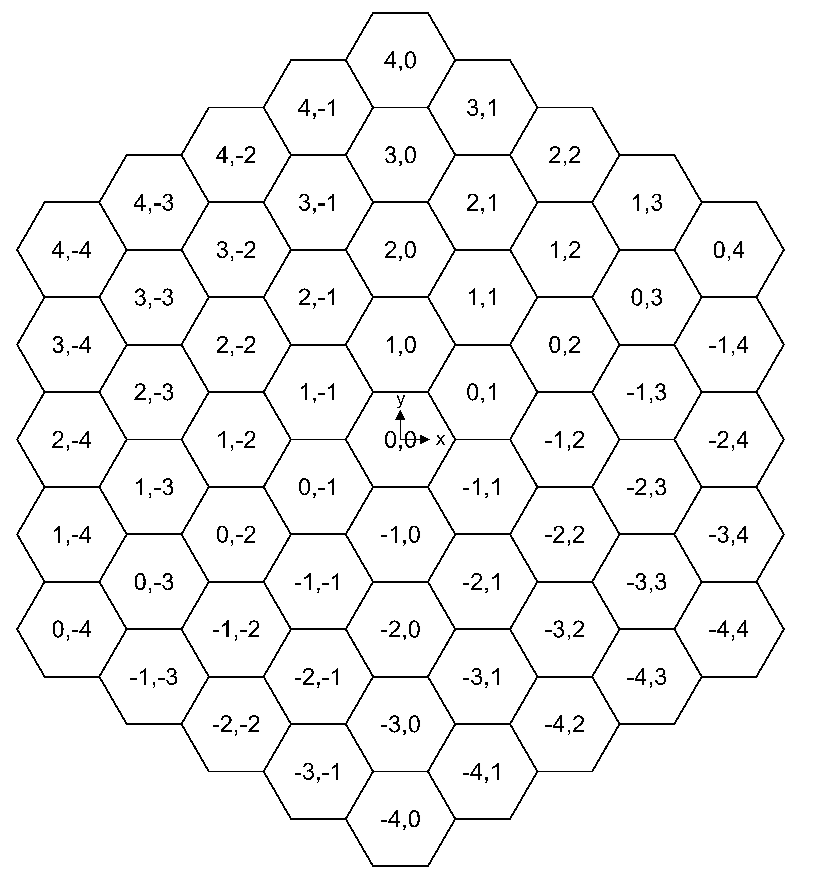
\includegraphics[width=0.34\textwidth]{HexagonIndices.png}
  \caption{Indizierung im \mbox{hexagonalen} Raster}
  \label{fig:hexindex}
\end{wrapfigure}
Da für eine effiziente Nutzung der Fläche des Erdsondenfeldes die einzelnen Erdsonden am besten in einem hexagonalen Raster platziert werden, ist es auch reizvoll, die Simulation der zweidimensionalen Wärmegleichung in einem hexagonalen Raster vorzunehmen. Ein hexagonales Raster stellt auch eine homogenere Aufteilung der Ebene dar.\\
Der Mittelpunkt oder Ursprung des hexagonalen Rasters hat den Index $(0,0)$. Die einzelnen Felder sind wie in Abbildung \ref{fig:hexindex} dargestellt indiziert. Die sechs Nachbarn des Feldes mit Index $(i,j)$ sind damit $(i-1,j+1)$, $(i,j+1)$, $(i+1,j)$, $(i+1,j-1)$, $(i,j-1)$ und $(i-1,j)$. Der kleine Durchmesser der Sechsecke sei $d$, was auch den Abstand der Mittelpunkte benachbarter Sechsecke definiert. Da ich keine Beschreibung eines solchen Verfahrens finden konnte, habe ich durch Ausprobieren und Vergleichen mit dem quadratischen Verfahren herausgefunden, dass die Temperaturdifferenz mit einem Faktor von $\frac{2}{3}$ ersehen werden muss, um das selbe Ergebnis zu liefern, wie das quadratische Verfahren. Somit ergibt sich für die explizite Form des Crank-Nicolson Verfahrens im hexagonalen Raster die folgende Form:
\begin{align}
T_{i,j}^{n+1}  = \frac{2}{3} \cdot \alpha \Delta t \cdot
\frac{T_{i-1,j+1}^n + T_{i,j+1}^n+ T_{i+1,j}^n+ T_{i+1,j-1}^n+ T_{i,j-1}^n+ T_{i-1,j}^n - 6T_{i,j}^n }{d^2}  + T_{i,j}^n
\end{align} 
Das Verfahren besteht auch alle Prüfungen wie oben beim quadratischen Verfahren beschrieben: Invarianz der Energie und gleiches Ergebnis bei feinerer Aufteilung der Zeitschritte und Sechseckgröße.
\subsubsection{Verfeinerung der Aufteilung an kritischen Stellen}
\begin{wrapfigure}{r}{0.35\textwidth}
  \centering
  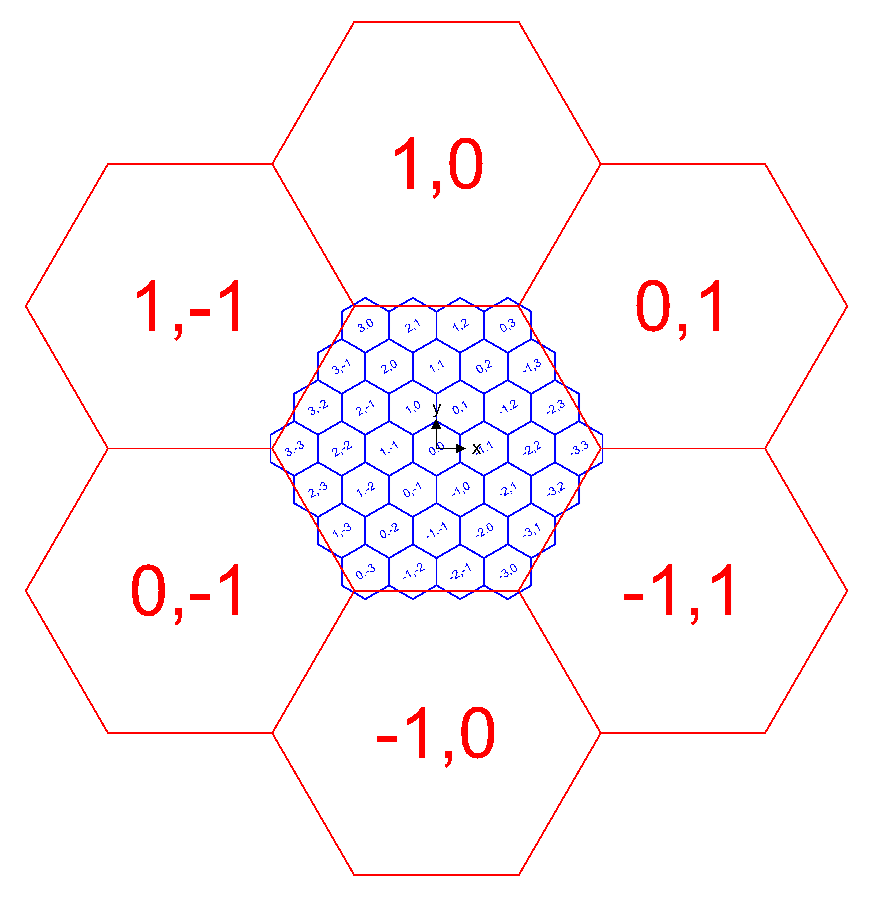
\includegraphics[width=0.34\textwidth]{HexagonSubdevide.png}
  \caption{Aufteilung eines Sechsecks in kleinere Sechsecke mit Indizierung}
  \label{fig:hexsubdevision}
\end{wrapfigure}
Die Stellen im Erdsondenfeld, an denen sich die Erdsonden befinden, stellen höhere Anforderungen an die Simulation als die Zwischenräume zwischen den Erdsonden. Für die räumliche Auflösung ist die Rasterung typischerweise so gewählt, dass in jeder Richtung fünf bis acht Sechsecke zwischen den mit Erdsonden bestückten Sechsecken liegen. Damit hat ein Sechseck einen Durchmesser in der Größenordnung von einem halben bis einen Meter. Die Erdsonden werden nicht im Detail so nachgebildet, dass die einzelnen Rohre und der umgebende Betonkern getrennt simuliert werden. Vielmehr soll das innerste Sechseck einer Unterteilung in etwa 15~cm groß sein, was in etwa dem Durchmesser einer Erdsondenbohrung entspricht. Die Leistung, mit der die Wärme vom durch die Erdsonde fließenden Wasser an den Bohrkern abgegeben wird, hängt von der Tiefe der Bohrung und dem Temperaturunterschied zwischen dem Wasser und dem Betonkern ab. Es ist eine Konstante mit der Einheit $\frac{W}{m \cdot K}$ Diese muss letztlich für jede Bauart abgeschätzt bzw. bestimmt werden.\\
Durch eine feinere Aufteilung des Sechsecks, welches eine Erdsonde enthält, kann das Verhalten in der Nähe der Erdsonde genauer simuliert werden.
\subsubsection{Randbedingungen}
Das Erdsondenfeld liegt natürlich nicht im luftleeren Raum, sondern ist seitlich, unten und oben im Kontakt mit der umgebenden Erdmasse.\\
Für die seitliche Randbedingung eignet sich ganz gut die Dirichlet Randbedingung: die Temperaturwerte am Rand werden auf einen bestimmten Wert "festgenagelt". Das macht weiter kein Problem, wenn man nur das zu simulierende Feld weit genug über die äußeren Erdsonden hinaus ausdehnt. Nach vielleich 50m außerhalb des Erdsondenfelds kann eine konstante Temperatur von 10~°C angenommen werden. Solange wir im Erdsondenfeld über dieser Temperatur liegen, rechnen wir damit mit größeren Verlusten als in Wirklichkeit.\\
Nach oben wird der Verlust dagegen ignoriert, da wir hier von einer Isolierung mit Schaumglas ausgehen, so dass die Verluste sehr gering ausfallen werden.\\
Bislang haben wir die Simualtion nur im zweidimensionaen betrachtet. In Wirklichkeit haben wir ja dreidimensionale Volumenelemente, in unserem Fall hexagonale Prismen, die typischerweise weniger als 1~m Durchmesser haben aber eine Länge von 100~m. Verdoppeln wir das Erdsondenfeld nach unten, so können wir den Wärmefluss von einem vertikalen Prisma in das zugehörige darunterliegende berechnen. Auch hier halten wir die Temperatur im "2. Untergeschoss" gemäß Dirichlet konstant, diesmal vielleicht bei 13~°C, da wir uns ja etwas tiefer in der Erde befinden.
\subsubsection{Grundwasserfluss}
Eine Bewegung des Grundwassers wird zur Zeit nicht berücksichtigt. Das ist sicherlich die größte Schwachstelle der Simulation. Letztlich bräuchte man den Volumenstrom des Grundwassers durch das Erdsondenfeld und ein Maß für die Wärmeübertragung zwischen Grundwasser und Erdmasse. Experimentell könnte man einen solchen Wert bestimmen, wenn wenigstens drei Bohrungen in einem gleichseitigen Dreieck vorliegen und man einen langen Thermal Response Test macht. 


\subsubsection{Verhalten bei Wärmezufuhr bzw. Wärmeentnahme} 
Die Temperaturänderung soll durch einen empirisch gewonnenen Faktor, der Sondenlänge und der Temperaturdifferenz zwischen der Erdsonde und dem die Sonde durchströmenden Wasser bestimmt werden. Für die nächste Sonde bei serieller Verbindung wird die durch die Energiezufuhr oder -entnahme veränderte Wassertemperatur verwendet.\\
Ein vorläufiger Test liefert zumindest anschaulich ansprechende Ergebnisse. Ob es gelingt, auf diese Art der gestellten Aufgabe gerecht zu werden, wird sich zeigen müssen.
\begin{figure}[h]
    \begin{minipage}[t]{.4\linewidth} % [b] => Ausrichtung an \caption
       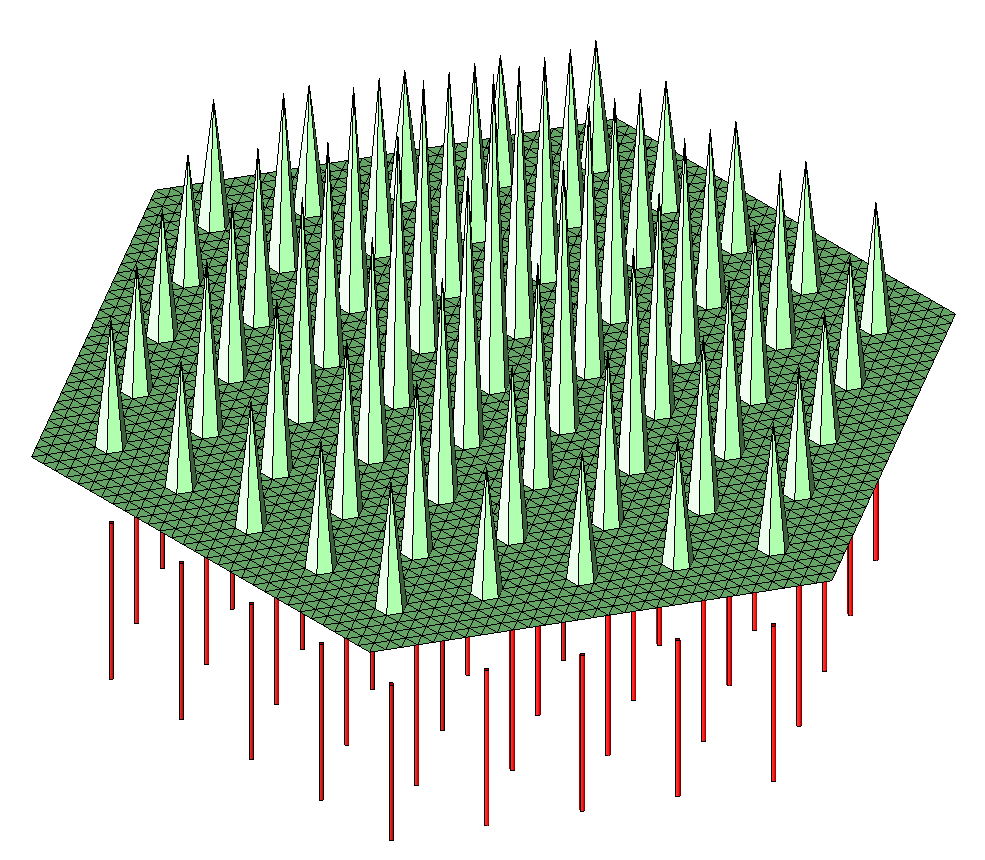
\includegraphics[width=\linewidth]{TempAt0.png}
       \caption{Temperaturverteilung unmittelbar nach Erwärmung durch die Edsonden}
       \label{TempAt0}
    \end{minipage}
    \hspace{.1\linewidth}% Abstand zwischen Bilder
    \begin{minipage}[t]{.4\linewidth} % [b] => Ausrichtung an \caption
       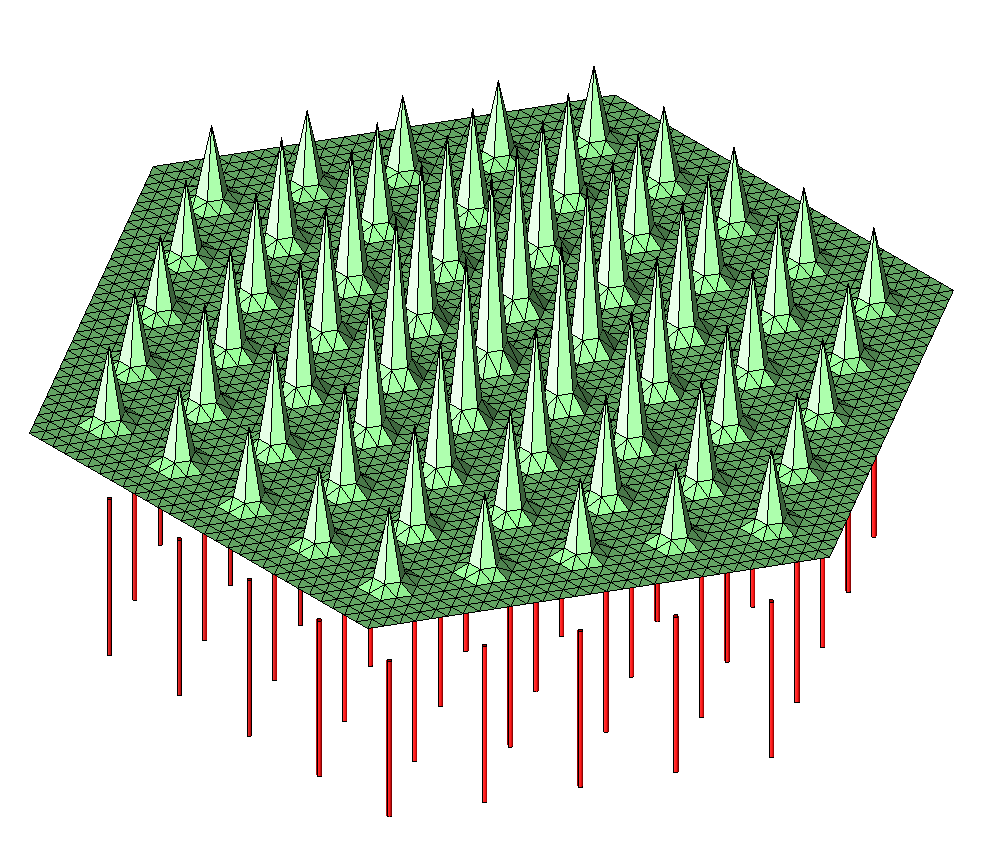
\includegraphics[width=\linewidth]{TempAt5.png}
       \caption{Temperaturverteilung kurze Zeit später}
       \label{TempAt5}
    \end{minipage}
 \end{figure}
 \begin{figure}[h]
    \begin{minipage}[t]{.4\linewidth} % [b] => Ausrichtung an \caption
       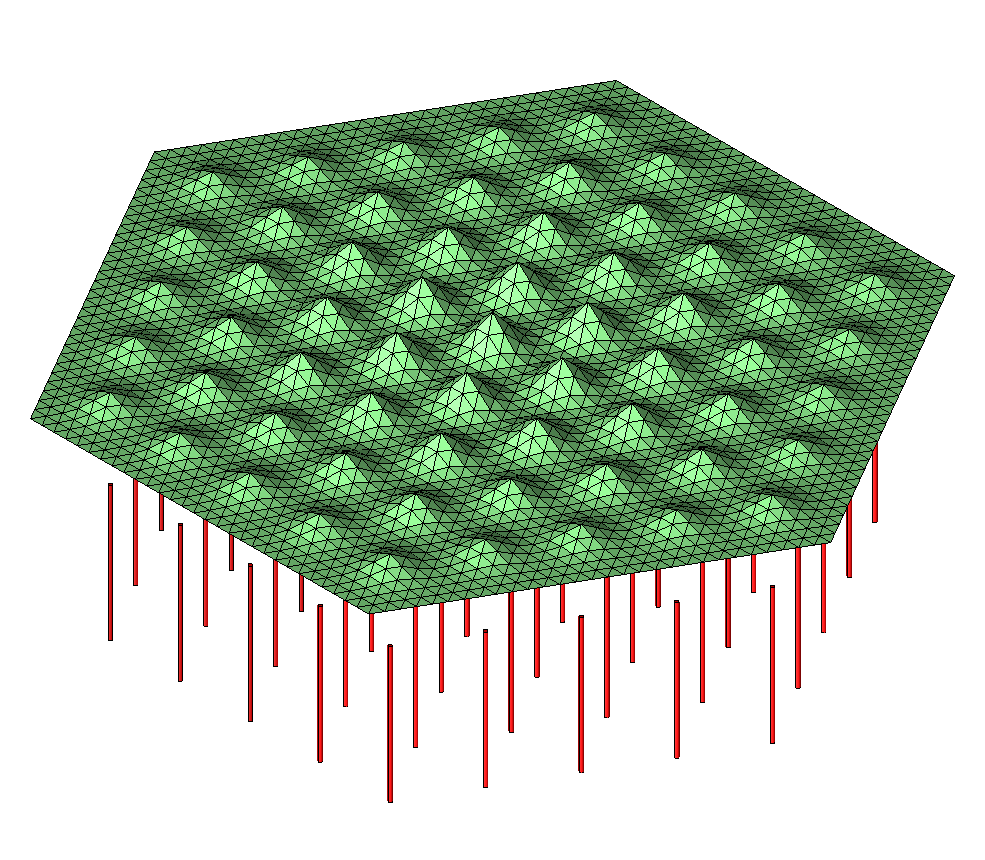
\includegraphics[width=\linewidth]{TempAt30.png}
       \caption{Temperaturverteilung nochmal später, die Erhöhung des Gesamtniveaus ist auf dem Bild kaum erkennbar}
       \label{TempAt30}
    \end{minipage}
    \hspace{.1\linewidth}% Abstand zwischen Bilder
    \begin{minipage}[t]{.4\linewidth} % [b] => Ausrichtung an \caption
       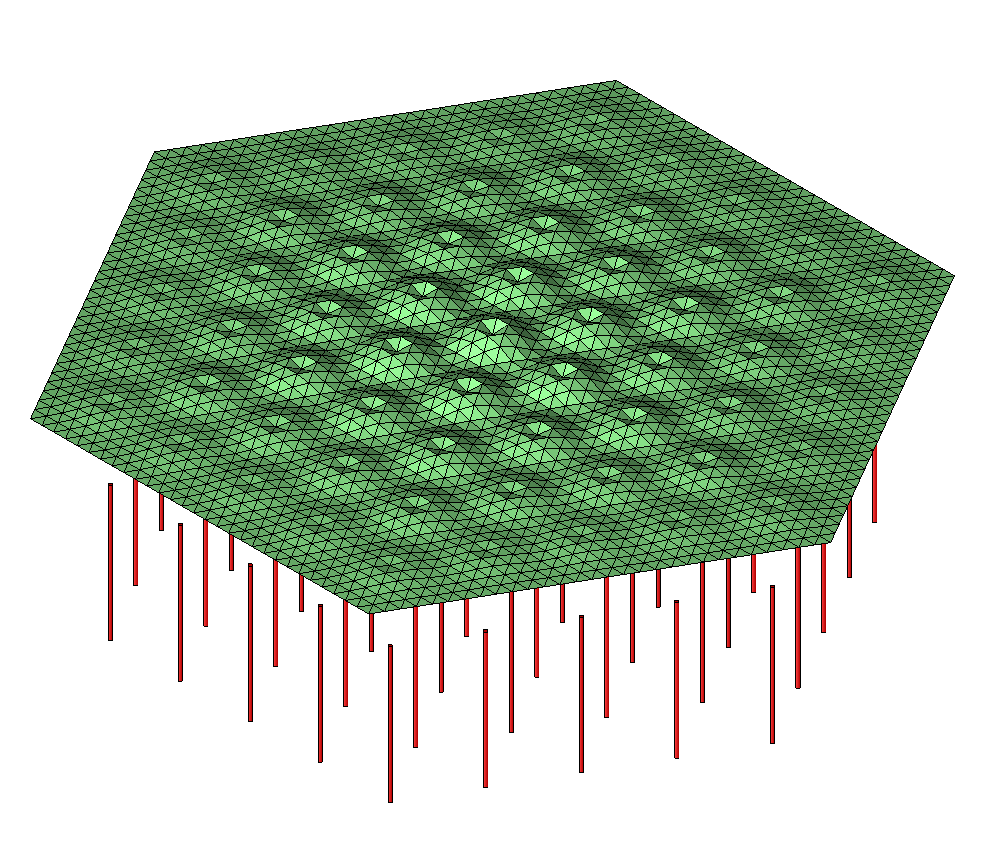
\includegraphics[width=\linewidth]{TempAt30m.png}
       \caption{Temperaturverteilung nachdem Wärme entnommen wurde}
       \label{TempAt30m}
    \end{minipage}
\end{figure}\\
Die Abbildungen \ref{TempAt0}, \ref{TempAt5}, \ref{TempAt30} und \ref{TempAt30m} zeigen das Temperaturprofil über den Erdsonden zu gewissen Zeitpunkten.
\end{document}
